\section{Model performance with Train/Test sets}
\label{ch:traintest}

To be more rigorous about judging model performance, and to avoid overfitting, we can fit our models using a \textit{training set} and evaluate it on new data in the \textit{test set}.

We will just display the plots for Ireland here for the sake of brevity.

\subsection{Summary}
Below is a summary of results of the applied model for the primary date range for the training set. The test set is then the following fourteen days.

\import{./}{Chapters/Ireland-summarydf.tex}
\import{./}{Chapters/Italy-summarydf.tex}
\import{./}{Chapters/United States-summarydf.tex}

Below is a summary of the parameters for the mathematical models, also located in the plots in the body of the report

\import{./}{Chapters/Ireland-mathmodelpars.tex}
\import{./}{Chapters/Italy-mathmodelpars.tex}
\import{./}{Chapters/United States-mathmodelpars.tex}

\subsection{Base Model}
\begin{figure}[H]
\minipage{0.48\textwidth}
  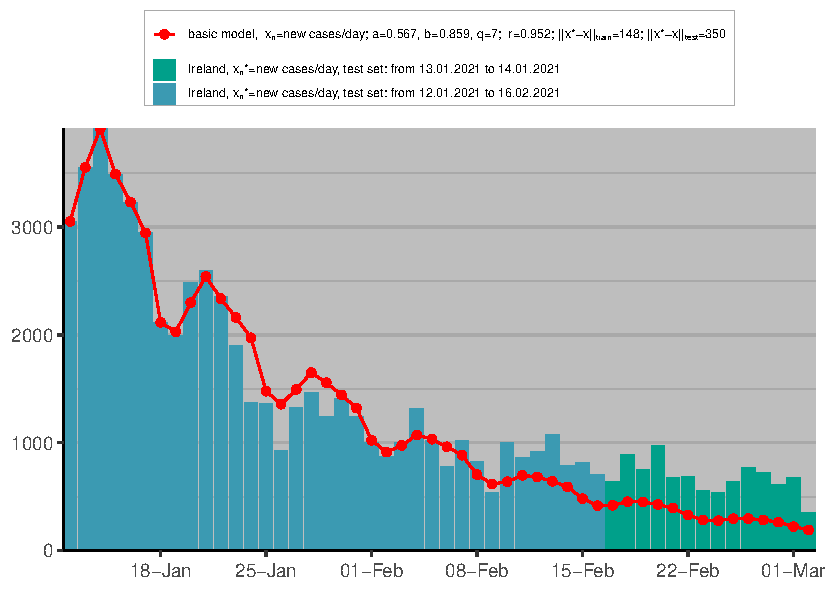
\includegraphics[width=\linewidth]{Ireland-basexn-traintest.pdf} \label{fig:ireland-basexn-traintest}
\endminipage\hfill
\minipage{0.48\textwidth}
  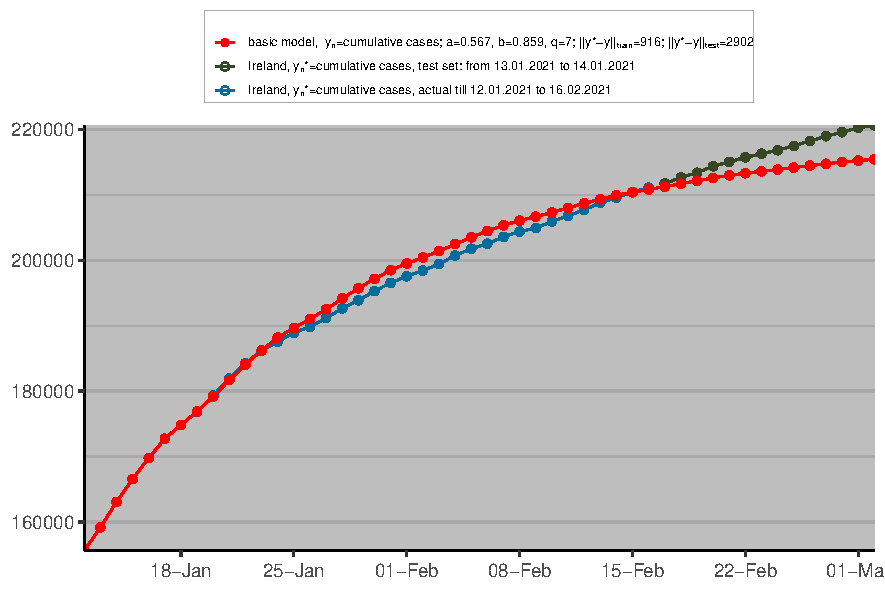
\includegraphics[width=\linewidth]{Ireland-baseyn-traintest.pdf} \label{fig:ireland-baseyn-traintest}
\endminipage
\caption{Basic model with train/test split, Ireland}
\end{figure}

\subsection{Periodic model}
\begin{figure}[H]
\minipage{0.48\textwidth}
  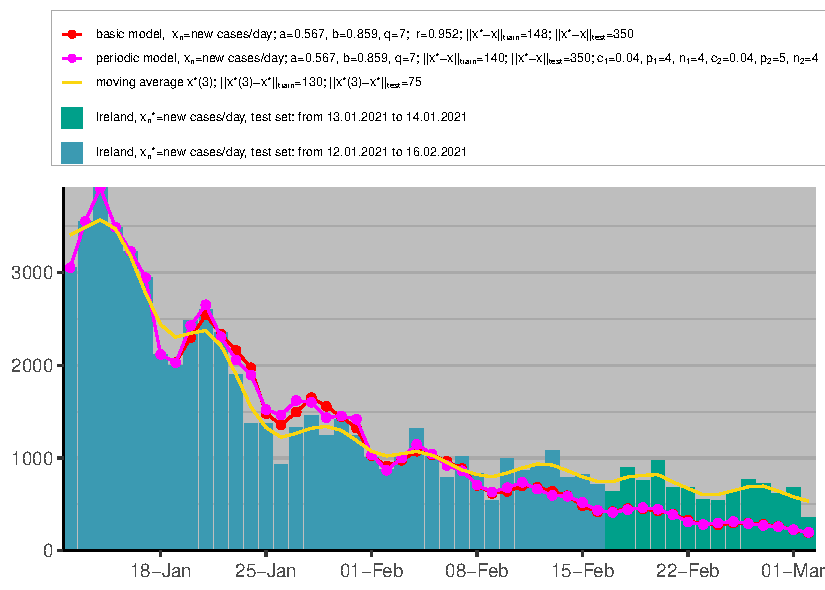
\includegraphics[width=\linewidth]{Ireland-periodic-traintest.pdf} \label{fig:ireland-periodic-traintest}
\endminipage\hfill
\minipage{0.48\textwidth}
  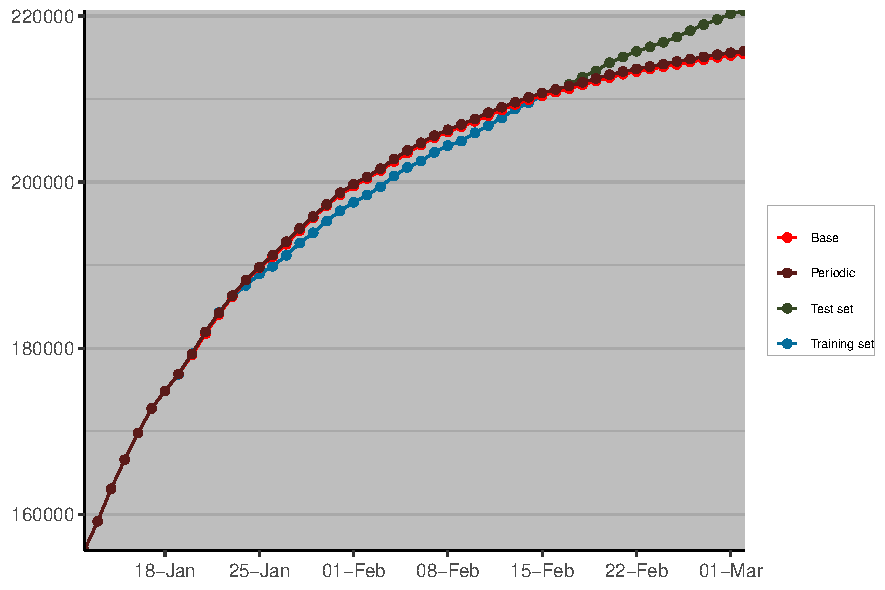
\includegraphics[width=\linewidth]{Ireland-periodicy-traintest.pdf} \label{fig:ireland-periodicy-traintest}
\endminipage
\caption{Periodic model with train/test split, Ireland}
\end{figure}



\subsection{HoltWinters model}
\begin{figure}[H]
\minipage{0.48\textwidth}
  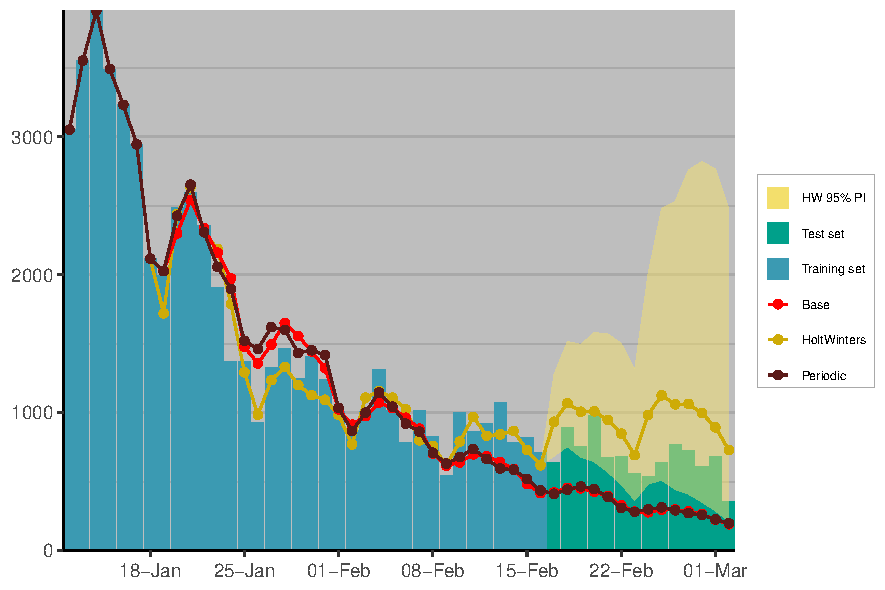
\includegraphics[width=\linewidth]{Ireland-hw-traintest.pdf} \label{fig:ireland-hw-traintest}
\endminipage\hfill
\minipage{0.48\textwidth}
  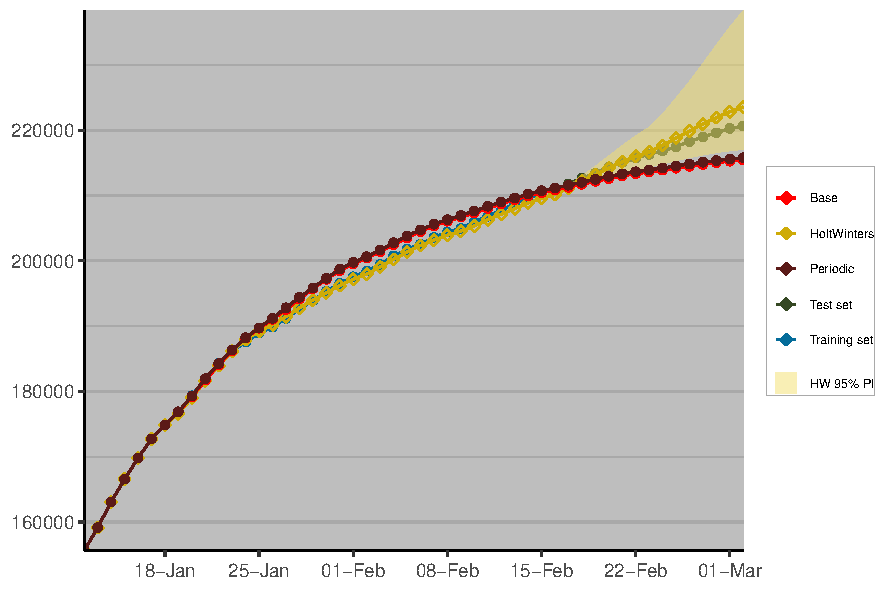
\includegraphics[width=\linewidth]{Ireland-hwy-traintest.pdf} \label{fig:ireland-hwy-traintest}
\endminipage
\caption{HoltWinters model with train/test split, Ireland}
\end{figure}


\subsection{ARIMA model}
\begin{figure}[H]
\minipage{0.48\textwidth}
  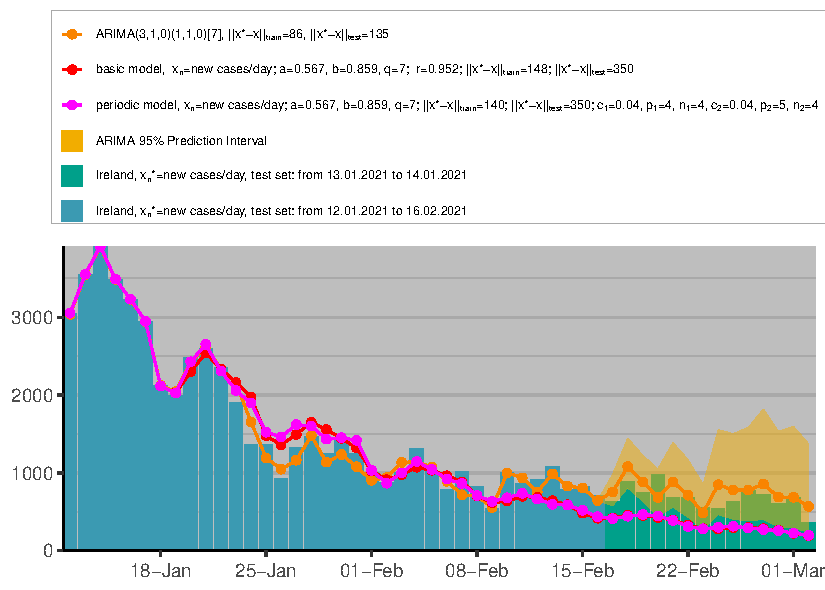
\includegraphics[width=\linewidth]{Ireland-arima-traintest.pdf} \label{fig:ireland-arima-traintest}
\endminipage\hfill
\minipage{0.48\textwidth}
  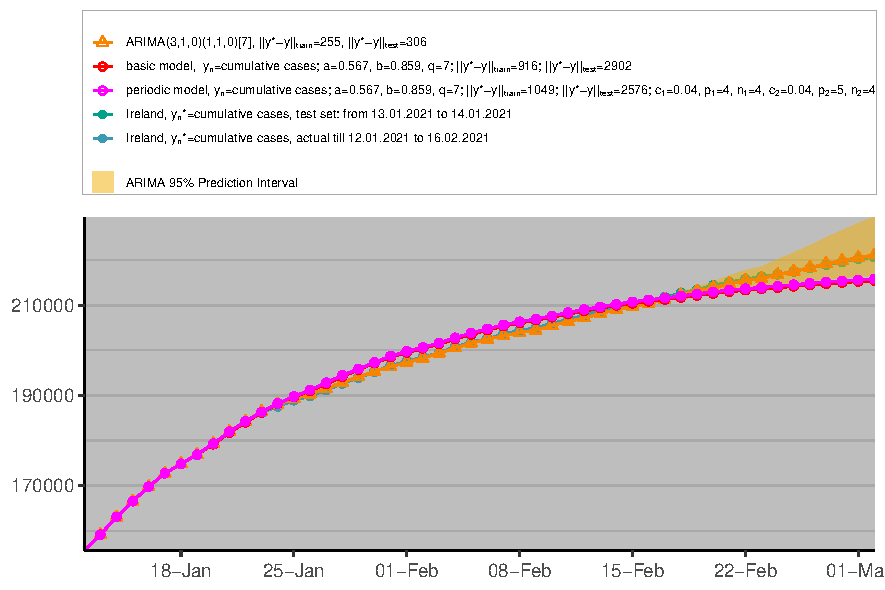
\includegraphics[width=\linewidth]{Ireland-arimay-traintest.pdf} \label{fig:ireland-arimay-traintest}
\endminipage
\caption{ARIMA model with train/test split, Ireland}
\end{figure}



\subsection{NNAR model}
\begin{figure}[H]
\minipage{0.48\textwidth}
  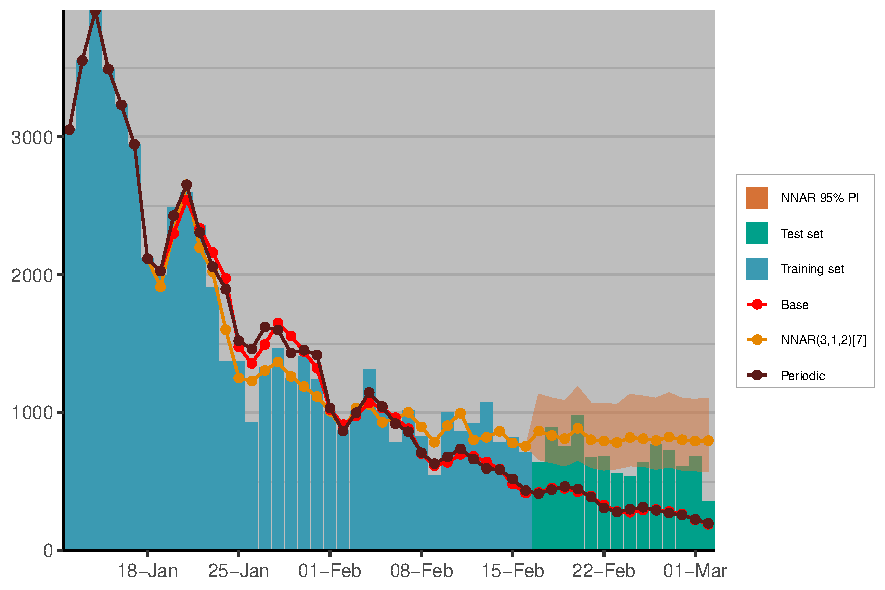
\includegraphics[width=\linewidth]{Ireland-nn-traintest.pdf} \label{fig:ireland-nn-traintest}
\endminipage\hfill
\minipage{0.48\textwidth}
  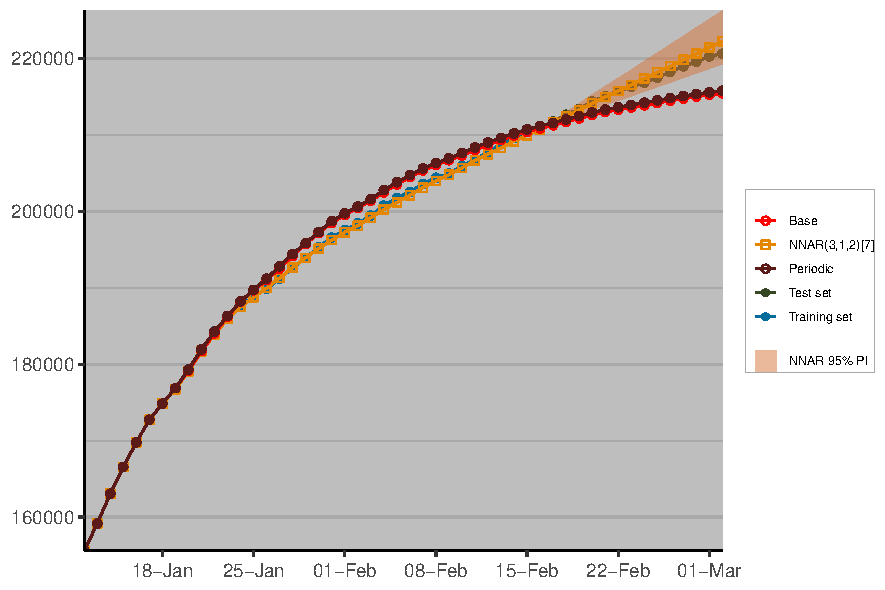
\includegraphics[width=\linewidth]{Ireland-nny-traintest.pdf} \label{fig:ireland-nny-traintest}
\endminipage
\caption{Neural Network Autoregression model with train/test split, Ireland}
\end{figure}